% main.tex - 科研项目学习笔记模板
% !TeX root = main.tex
%%%%%%%%%%%%%%%%%%%%%%%%%%%%%% DOCUMENT 
\documentclass[12pt]{report}

%%%%%%%%%%%%%%%%%%%%%%%%%%%%%% PACKAGES

% 中文支持(XeLaTeX 编译)
\usepackage[UTF8]{ctex}
\usepackage{xeCJKfntef} 

% \setCJKmainfont{HanziPen SC}
% \setmainfont{HanziPen SC}


% 页面设置
\usepackage[a4paper, left=20mm, right=20mm, top=15mm, bottom=15mm]{geometry}

\PassOptionsToPackage{dvipsnames,svgnames,x11names}{xcolor}
\usepackage{xcolor}


% 数学环境及符号
\usepackage{amsmath, amssymb, amsfonts, amsthm,amsopn}
\usepackage{tensor}              % 张量指标管理
\usepackage{mathtools}           % amsmath增强
\usepackage{physics}             % 物理公式快捷命令
             % Dirac符号
\usepackage{bbold}               % 数学黑体
\usepackage{dsfont}              % 另一种数字体
\usepackage[mathscr]{eucal}     % 花体字母
\usepackage{tensor}              % 张量指标管理
\usepackage{simpler-wick}       % Wick记号
\usepackage{mathrsfs}            % 另一种花体字母

% 颜色与图形相关
\usepackage{graphicx}           % 插图支持
\usepackage{float}              % 浮动体控制
\usepackage{tikz}               % 绘图库
\usetikzlibrary{math}           % tikz数学扩展
\usepackage{geometry}
% 表格与列表
\usepackage{makecell}           % 表格多行换行
\usepackage{multicol}           % 多栏排版
\usepackage{colortbl}           % 表格颜色
\usepackage{enumitem}           % 列表自定义

% 其他辅助
\usepackage{framed}             % 有边框环境
\usepackage{tcolorbox}          % 灵活盒子环境
\tcbuselibrary{breakable}       % 盒子内容分页
\usepackage{thmtools}           % 定理环境管理
\usepackage{thm-restate}        % 定理重述
\usepackage{showlabels}         % 显示标签,调试用(完成后可注释)
\usepackage[normalem]{ulem}     % 下划线、删除线
\usepackage{hyperref}           % 超链接(最后加载)
\usepackage{cleveref}           % 智能引用(紧跟hyperref)
\usepackage{soul}

% 自定义宏包
\usepackage{macros}

% 一个中文可以高亮的包
\usepackage{cjkhl}
\definecolor{lightblue}{rgb}{.8,.8,1}

%%%%%%%%%%%%%%%%%%%%%%%%%%%%%% 自定义命令
\newcommand{\tml}{Teichmüller space}
\newcommand{\hil}{Hilbert space}
\newcommand{\mtc}{Modular Tensor Category}

%%%%%%%%%%%%%%%%%%%%%%%%%%%%%% BEGINNING OF THE DOCUMENT

\begin{document}

\title{\boldmath Modern approach Quantum Gravity note}
\author{X. D. H.}

\maketitle

\begin{abstract}
  这个笔记是2025年秋天liuy旁听Monica的Modern approach to Quantum Gravity课程时做的笔记。由于此时liuy物理水平还有限,所以需要课下补充很多preliminary的东西,也比较乱。

  由于课程风格是上课讲的比较随意。很多细节推导需要课后补充。所以笔记中会补充很多很多很多的内容。基本以monica的授课作为主线很多参考书进行补充捏。
\end{abstract}

\tableofcontents

\chapter{Lecture 1}
\section{Take home messages}\label{sec:Take home messages} % (fold)
\imp{总论}{

  Lecture之中。我们回顾了Poincare群的结构以及其表示理论。根据表示理论得到了一些基量子态。然后根据不同的Lorantz Transformation的变换把这些量子态变换到不同的一般基之中。介绍了 normal basis, spin basis, helicity basis 的性质。
}

\subsection{Poincare Group and Representation}

我们狭义相对论研究的是不同惯性系之间的物理规律是不变的。那么说明,我们需要研究惯性系之间物理量是怎么变换的。变换构成了poincare group ISO(3,1):
\begin{equation}
  x^{\prime\mu} = g(\Lambda, a) x^\mu =\Lambda^\mu{}_{\nu}x^\nu+a^\mu,\quad\Lambda\in SO(3,1),\quad a\in\mathbb{R}^4. 
  \label{eq:poincaregroup}
\end{equation}

对于这个群来说满足下面的性质:
\begin{equation}
  \begin{aligned}&g(\Lambda_1,a_1)g(\Lambda_2,a_2)=g(\Lambda_1\Lambda_2,\Lambda_1a_2+a_1),\\&g(\Lambda,a)=g(1,a)g(\Lambda,0),\\&g^{-1}(\Lambda,a)=g(\Lambda^{-1},-\Lambda^{-1}a).\end{aligned}
  \label{eq:poincareproperty}
\end{equation}
下面我们考虑量子力学的Hilbert Space里面。这个群所有元素可以通过生成元进行exp map给出来:
\begin{equation}
  \begin{aligned}
  &U(g(\Lambda,0)) = U(\Lambda)=\exp(-\frac{i}{2}\omega_{\mu\nu}\mathcal{J}^{\mu\nu}),\\&U(g(0,a)) = U(a)=\exp(ia_\mu P^\mu).
  \end{aligned}
  \label{eq:groupele}
\end{equation}

我们发现这个群的表示是有下面的generator并且满足这样的对易关系:
\begin{equation}
  \begin{aligned}&[P^\mu,P^\nu]=0,\\&[P^\mu,\mathcal{J}^{\rho\sigma}]=i(\eta^{\mu\rho}P^\sigma-\eta^{\mu\sigma}P^\rho),\\&[\mathcal{J}^{\mu\nu},\mathcal{J}^{\rho\sigma}]=i(\eta^{\nu\rho}\mathcal{J}^{\mu\sigma}+\eta^{\mu\sigma}\mathcal{J}^{\nu\rho}-\eta^{\mu\rho}\mathcal{J}^{\nu\sigma}-\eta^{\nu\sigma}\mathcal{J}^{\mu\rho}),\end{aligned}
  \label{eq:generator}
\end{equation}

并且我们根据exp map以及群的乘法关系我们发现生成元都是tensor operator并且满足变换关系:
\begin{equation}
  \begin{aligned}&U^\dagger(a)P^\mu U(a)=P^\mu,\\&U^\dagger(\Lambda)P^\mu U(\Lambda)=\Lambda_\nu^\mu P^\nu,\\&U^\dagger(\Lambda)\mathcal{J}^{\mu\nu}U(\Lambda)=\Lambda_\rho^\mu\Lambda_\sigma^\nu\mathcal{J}^{\rho\sigma}.\end{aligned}
  \label{eq:transform}
\end{equation}
为了构建表示,我们需要选择Casimir Operator,并且用Casimir Operator的本征子对于空间进行分类。Casimir是Poincre Inv的算符,我们发现是:
\begin{equation}
  M^2=P^\mu P_\mu \quad W^2=W^\mu W_\mu 
  \label{eq:casimirpoincare}
\end{equation}
其中$ W^\mu = \displaystyle\frac{1}{2}\varepsilon^{\mu\nu\rho\sigma}P_\sigma \mathcal{J}_{\nu\rho} $是Pauli-Lubanski矢量。所以我们的Hilbert Space可以写作;
\begin{equation}
  \mathcal{H}=\bigoplus_{m^2,w^2}\mathcal{H}(m^2,w^2).  
  \label{eq:Hilbertspace}
\end{equation}
所以我们不妨在固定一个$ m^2, w^2 $考虑量子态$ \ket{p,\sigma} $,发现这样的量子态有四类,并且每一类都可以通过一个特殊向量给出,并且这个基向量的不变的群元素定义了一个little group,我们知道$ \sigma $就是应该label这一部分的:

\begin{figure}[H]
  \centering
  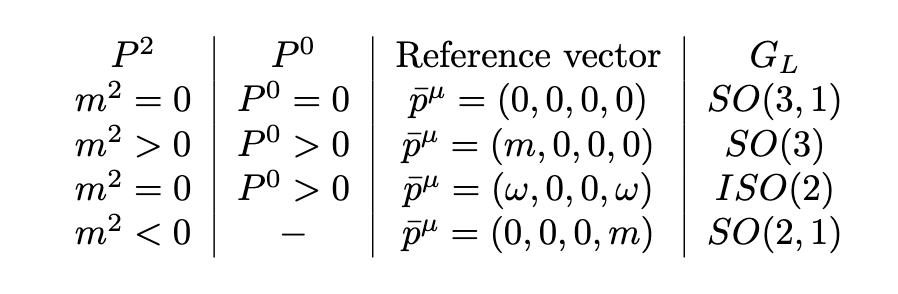
\includegraphics[width=0.55\textwidth]{assets/littlegroup.png}
  \label{fig:littlegroup}
\end{figure}
一个结论是除了真空(第一个)之外我们发现P-L Tensor正好构成了这个little group的生成元。证明方法是直接计算$ W^\mu $作用 $ W^\mu \ket{\bar{p},\sigma} = \displaystyle\frac{1}{2} \epsilon^{\mu\nu\rho\sigma} \bar{p}^\sigma \mathcal{J}^{\nu\rho} \ket{\bar{p}, \sigma}$。我们会发现这些分量作用根本不改变$ \bar{p} $。所以这些量是little group的生成元。





% section Take home messages (end)

\section{Questions and discussions}\label{sec:Questions and discussions} % (fold)

\question{ 为什么只有洛伦兹变换可以有很完善的$ \tensor{J}{^\mu_a} $,为什么不是poincare group?}

注意!我们对于张量的$ \tensor{\Lambda}{^\mu_a} $的定义其实是$ \displaystyle\frac{dx^\mu}{dy^a} $所以我们poincare变换在求导之中平移变换就没了!!

\question{ 算符的升降指标意味着什么?张量算符的协变形式思考一下!}

当我们讨论张量算符的升降指标的时候。我们想说的是张量算符的升降指标会不会意味着会改变Poincare Group的Unitary算符作用在这个算符两端给出的结果是逆变的。显然是这样的捏。我们可以认为升降指标就是作用上一个metric,metric作用在$ \Lambda^\mu{}_\nu $上面会变成逆变的。 

\question{ $ \Lambda^\mu{}_a $ LT的逆矩阵的指标前后,到底怎么写捏?}

$ (J^{-1})^{\nu}{}_{a} = J^\nu{}_a$ 这是一个很好的记号捏捏。课上老师写的$ (\Lambda^{-1})_\mu{}^{\nu} $应该是很错误的写法!!

我们还需要讨论洛伦兹变换矩阵如果升降指标会发生什么:
\begin{equation}
  \Lambda^{-1\mu}{}_a = \Lambda_\mu{}^a
  \label{eq:inverseandlift}
\end{equation}
这个就是Rattazzi混淆的地方捏。


\question{ 为什么动量,角动量算符什么的是和表示的生成元是一样的呢?怎么证明?}


\question{ 为什么构成的Lorentz Inv Scalar 只有四个独立的呢?}

这里我们讨论的是从洛伦兹生成元构成的洛伦兹不变量独立的个数。这个讨论虽然是量子的,但是我们知道洛伦兹变换的生成元都是对于洛伦兹变换的张量算符:
\begin{equation}
  \begin{aligned}&U^\dagger(\Lambda)P^\mu U(\Lambda)=\Lambda_\nu^\mu P^\nu,\\&U^\dagger(\Lambda)\mathcal{J}^{\mu\nu}U(\Lambda)=\Lambda_\rho^\mu\Lambda_\sigma^\nu\mathcal{J}^{\rho\sigma}.\end{aligned}
  \label{eq:tensoroperator}
\end{equation}
所以,这些量就仿佛是量子化后的客观测量一样。并且量子化后的变换和经典的是一毛一样的,我们不妨把这些可观测量当成经典的来构造lorantz invariant。

我们把$ \mathcal{J^{\mu\nu}} $本身理解为一个物理量。这个物理量是对于lorentz协变的。我们考虑这个物理量到底有哪些自由度。我们会发现,如果换一个惯性系「或者说进行lorentz变换」可以变到一个canonical form:
\begin{equation}
 J_{\mathrm{canonical}}^{\mu\nu}=\begin{pmatrix}0&-E&0&0\\E&0&0&0\\0&0&0&-B\\0&0&B&0\end{pmatrix} 
  \label{eq:canonicalformofJ}
\end{equation}
我们现在意识到这个量独立的自由度只有两个:$ E $和$ B $。所以我们可以构造两个独立的lorentz invariant 其实只有两个。最后得出的结论是:
\begin{equation}
  \mathcal{J}^{\mu\nu}\mathcal{J}_{\mu\nu},\mathrm{~}\varepsilon^{\mu\nu\rho\sigma}\mathcal{J}_{\mu\nu}\mathcal{J}_{\rho\sigma}
  \label{eq:indep}
\end{equation}
这两个算符其实是Lorentz Group的Casimir Operator。

并且有意思的是,这个有一些电动力学的影子。因为$ \mathcal{J}^{\mu\nu} $在洛伦兹群下面的变换关系和电磁场张量$ F^{\mu\nu} $在洛伦兹群下面的变换关系是一样的。所以,我们也就发现,用电磁场张量构造的两个不变量也是两个独立的Lorentz Invariant。其中第一个的物理意义就是$ E^2-B^2 $,第二个物理意义是$ \vec{E}\cdot\vec{B} $。第一个不变量就是电磁场的Lagrangian。


但是还没有完,这个是$ \mathcal{J}^{\mu\nu} $矩阵的情况,我们还需要考虑$ P^\mu $。我们会发现能够构造的独立的Lorentz Invariant (带上P)其实是四个:\begin{equation}
  P^{\mu}P_{\mu},\mathcal{J}^{\mu\nu}\mathcal{J}_{\mu\nu},\varepsilon^{\mu\nu\rho\sigma}\mathcal{J}_{\mu\nu}\mathcal{J}_{\rho\sigma},W^{\mu}W_{\mu},
  \label{eq:fourinvariant}
\end{equation}

对于两个带P的我没有什么直观的理解呀呀呀,希望之后能补充一下。


\question{ Little group之中使用的 $ \Lambda_k $和 一般Lorentz trans $ \Lambda  $什么关系?}

我目前绝地就是完全是一个lorantz group里面的一个东西。问题出在哪里呢,出在我们定义不同的basis的时候使用了定义式(比如对于normal basis我们有):
\begin{equation}
  \ket{k,\sigma} = U(\Lambda_k)\ket{\bar{p},\sigma}
  \label{eq:definebasis}
\end{equation}
我们这个量子态的$ \ket{k,\sigma} $之中的$ \sigma $指的是在$ U(\Lambda_k) $转动之前是$ \sigma $。或者就是指从$ \ket{\bar{p},\sigma} $转动过去的!
% section Questions and discussions (end)
 

\chapter{Scratch Book}
\sout{这里会放一些写的很混沌,但懒得扔掉的东西呜呜呜呜!!!}



\end{document}
